\documentclass{css}
%\documentclass[english]{css}

\usepackage[dvips]{graphicx}
\usepackage{latexsym}

\def\|{\verb|}

\newcommand{\cssyear}[0]{2023}
\newcommand{\cssname}[0]{CSS 2023}
\newcommand{\cssversion}[0]{2023/06/01}
\newcommand{\cssemail}[0]{css2023-office@iwsec.org}

\begin{document}

%% 本文が和文の場合,タイトル・著者名・著者所属・概要は,和文・英文共に必須.
%% If you prepare this manuscript in English, there is no need to put Japanese metadata (title, author names, affiliations, abstract, and keywords) in it.

\title{Isolation Forestを用いた\\IoT向け異常検知手法に関する考察}
\etitle{A Study on Anomaly Detection Method \\for IoT using Isolation Forest}

\affiliate{XX}{東京工業大学 情報理工学院 数理・計算科学系\\
Department of Mathematical and Computing Sciences, School of Computing, Tokyo Institute of Technology}
\affiliate{YY}{株式会社YYセキュリティ研究所\\
Security Laboratories, YY Corporation}
\paffiliate{ZZ}{国立研究開発法人ZZ研究所\\
National Institute of ZZ}

%% メールアドレスは省略可能だが,代表者のメールアドレスは必須.
%% 姓名の間は半角スペースを入れること.

\author{菅田 大輔}{Daisuke Sugata}{XX}[sugata.d.aa@m.titech.ac.jp]
\author{石井 将大}{Masahiro Ishii}{XX, YY, ZZ}[]
\author{松浦 知史}{Satoshi Matsuura}{YY}[]

%% the following is author command for english option.
%% at least one e-mail address is required.

%\author{Taro Joho}{XX}[taro.joho@xx.ac.jp]
%\author{Hanako Anzen}{XX, YY, ZZ}

\begin{abstract}
    本論文では、Isolation Forestを用いたIoT向け異常検知手法の改善を行なった。この研究の背景にIoT(Internet of Things)の普及がある。2030年には約300億台ものデバイスが利用されると予測されており、すべてのIoT機器のセキュリティ確保が重要な課題となっている。特に2016年のMirai型マルウェアによるDDoS攻撃はその必要性を浮き彫りにした。本研究は専門的なセキュリティ対策が難しい、家庭内ネットワークなどの小規模環境に着目し、軽量で高速な異常検知システムの提案を目指した。Isolation Forestは軽量で高速に動作する異常検知手法として注目されているが、これを用いた従来の方法には二つの問題が存在する。閾値を手動で設定する必要がある点と、閾値による異常判定のアルゴリズムの精度に限界がある点である。これらの課題を解決するため、異常判定をする際にロジスティック回帰を応用した判定アルゴリズムを提案する。提案手法を二つのデータセットで実験した結果、精度がそれぞれ84.4\%から91.1\%、84.6\%から94.5\%に改善したことを確認した。
\end{abstract}

%% キーワード (1--5単語) の記載は任意.

\begin{jkeyword}
Isolation Forest, IoT, IDS, 異常検知
\end{jkeyword}

\begin{eabstract}
    This paper presents an improved anomaly detection method for IoT environments using Isolation Forest. The motivation for this study lies in the widespread adoption of the Internet of Things. By 2030, it is estimated that around 30 billion devices will be in use, making the security of all IoT devices a critical issue. The necessity of this was highlighted by the 2016 DDoS attack caused by Mirai malware. This study focuses on small-scale environments, such as home networks, where implementing specialized security measures is challenging, and aims to propose a lightweight and fast anomaly detection system. Although Isolation Forest is recognized for being a lightweight and fast anomaly detection method, traditional approaches using it have two main issues: the need for manual threshold setting and limitations in the accuracy of anomaly detection algorithms based on these thresholds. To address these challenges, we propose an anomaly detection algorithm that incorporates logistic regression for decision-making. Experiments on two datasets showed that the accuracy of the proposed method improved from 84.4\% to 91.1\% and from 84.6\% to 94.5\%, respectively.
\end{eabstract}

%% the following keyword part is optional and can be omitted.

\begin{ekeyword}
Isolation Forest, IoT, IDS, Anomaly Detection
\end{ekeyword}

%% if you use english opsion, you should put your English abstract in the abstract environment.
%% eabstract is not displayed in english mode.

\maketitle

%1
\section{はじめに}
Isolation Forest(以下、IF)は、その計算効率の良さから異常検知に広く用いられている。AbuAlgahamらは、IoT向けのIDS(Intrusion Detection System)としてIFを用いた手法を提案している。しかし、IFを用いた従来の手法には、手動での閾値設定や判定精度の限界など、いくつかの課題を抱えている。本研究では、これらの問題に対処するために、IFの異常判定にロジスティック回帰を応用した新たな異常検知手法を提案する。
この研究の背景として、IoT(Internet of Things)の急速な普及が挙げられる。実際\ref{}によると、2030年には約300億台ものデバイスが利用されると予測されており、すべてのIoT機器のセキュリティ確保が重要な課題となっている。特に2016年のMirai型マルウェアによるDDoS攻撃はその必要性を浮き彫りにした。GitHub, Twitter, Reddit, Netflixなど, いくつかの有名ウェブサイトがアクセス不能になった. これは、家庭用のルーターやデジタルビデオレコーダーなどの管理不十分なデバイスが Mirai型マルウェアに感染し, 一斉に特定のサーバーにアクセスを行うよう強制されたことが原因である.
公的機関や企業組織といった大規模な環境では, セキュリティの専門家が構築し運用するフレームワークによって, IoT機器の安全性が確保されている. しかし, 先ほど述べたように、IoT機器は多くの場所で使用されており, 家庭内のネットワークなどの小さな組織の場合となると, これらを管理・運用するための人員リソースを確保するのが難しくなる. 加えて、高価なセキュリティシステムを導入することも困難である. そのため, 安価な計算機環境でも高速に動作するようなセキュリティシステムが求められている.
こうした背景から, 小規模な環境に適した IDS (Intrusion Detection System) の設計について考察する. 3章で従来の IF を用いた異常検知手法の問題点を整理し, 4章でこれらの問題を解決する提案手法について述べる. 5章では, UNSWとNSLの2つのデータセットを用いて、提案手法の有効性を評価した.

\section{研究方法}

\subsection{Isolation Forestの説明}

Isolation Forest(以下、IF)は、外れ値を効率的に検出するためのアルゴリズムである。この手法は、異常データが全体のデータセット中で数が少なく、他の正常データから離れて存在するという特性に基づいて設計されている。データをランダムに分割していく過程で、異常データは正常データに比べて相対的に早く孤立するため、データが孤立するまでに必要な分割回数に着目することで、異常データを検出できる。IFの実行は以下のステップに分かれる。

\subsubsection{データの分割}

IFは、ランダムに選んだ特徴量を基にデータを分割する。具体的には、選んだ特徴量のランダムな値を閾値として使用し、その閾値より大きいグループと小さいグループにデータを二分割する。この分割を全てのデータが孤立するまで繰り返し行い、一つの決定木(ITree)を作成する。このプロセスが終了したら、複数の決定木を構築する。

\subsubsection{異常スコアの算出}

異常スコアは、データ点が生成されたiTreeの枝をたどって到達するまでのパス長に基づいて計算される。パス長が短いほど、そのデータ点は異常である可能性が高い。異常スコア$V(x,n)$の計算式は式\ref{eq:anomaly_score}の通りである。


\begin{equation}
    V(x, n) = 2^{-\frac{E(h(x))}{c(n)}}
    \label{eq:anomaly_score}
\end{equation}


ここで、E(h(x)) はデータ点 x の平均パス長、c(n) はデータセットのサイズ n に依存する調整用の定数である。

\subsubsection{異常判定}

計算された異常スコアを使用して、異常検知を行う。一般的には、トレーニングデータにおける異常スコアの上位10\%を閾値として設定する。この閾値を超えるスコアを持つデータは異常と判定される


\subsection{IDSの概要}
本研究では、小規模なIoT環境に適したIntrusion Detection System(IDS)の設計について検討する。具体的には、Isolation Forestを用いた異常検知手法が提案され、その有効性を評価する。

\subsection{全体の設計}
IDSの設計は以下の3つのセクションに分けられる
\begin{enumerate}
    \item \textbf{データの前処理}
        \begin{itemize}
            \item 入力データを適切な形式に変換する。
            \item 不必要な特徴量の削除やデータの標準化、ラベルエンコーディングを行う。
        \end{itemize}
    \item \textbf{特徴量選択}
        \begin{itemize}
            \item 判定に重要な特徴量を選択し、過学習を防ぎ、検知精度を向上させる。
            \item Random Forestを用いて特徴量の重要度を算出し、重要な特徴量を選択する。
        \end{itemize}
    \item \textbf{異常判定}
        \begin{itemize}
            \item IFを用いて通信が攻撃通信であるかを判定する。
            \item 特徴量の選択後、Isolation Forestで異常検知を行う。
        \end{itemize}
\end{enumerate}

\subsection{実装}

実装は以下のステップで行われる。

\subsubsection{データの前処理}

実装の初段階では、判定に不適切な特徴量、例えば時間やIPアドレスなどの無関係な特徴量を削除する。次に、Isolation Forestが数値データのみを入力として受け付けるため、カテゴリカルデータを数値データに変換する必要がある。この変換にはone-hotエンコーディングを利用し、異なるカテゴリの特徴を個別の数値特徴として表現する。さらに、データセットは攻撃データと正常データに事前に分割され、それぞれ別のデータセットとして扱われる。

\subsubsection{特徴量選択}

特徴量選択はRandom Forestアルゴリズムを使用して行われる。このプロセスでは、特徴量の重要度が算出され、重要度が設定された閾値を超える特徴量のみが選択される。この選択により、モデルの性能に直接影響を与える重要な特徴量を維持し、過剰適合を防ぐために不必要な特徴量は排除される。

\subsubsection{異常判定}

攻撃の判定では、IFを用いて攻撃通信と正常通信のデータに対して別々にトレーニングを行う。この2つのIFをサブシステムと呼ぶ。トレーニング後、それぞれのデータに対して異常スコアが算出される。異常スコアは、データがどの程度異常であるかを定量的に表す指標であり、最終的な判定は2つのサブシステムからの出力を組み合わせることで行われる。


\section{Isolation Forestの問題点の整理}
IFを異常検知手法として使用する際にどのような問題があるのかを明らかにするための事前実験を行った.はじめにデモデータを使用して,IFの挙動を確認し,その考察をもとに特徴量選択手法の提案を行なった.

\subsection{ノイズ特徴量が混入すると精度が悪化する問題}
使用するデモデータは、(2.5, 2.5)と(-2.5, -2.5)を中心とした
正常データ群と、10から-10の範囲に一様に分布した異常データ群からなる.二次元の場合のデモデータを図\ref{fig:demodata}に示す.

\begin{figure}[tb]
    \centering
    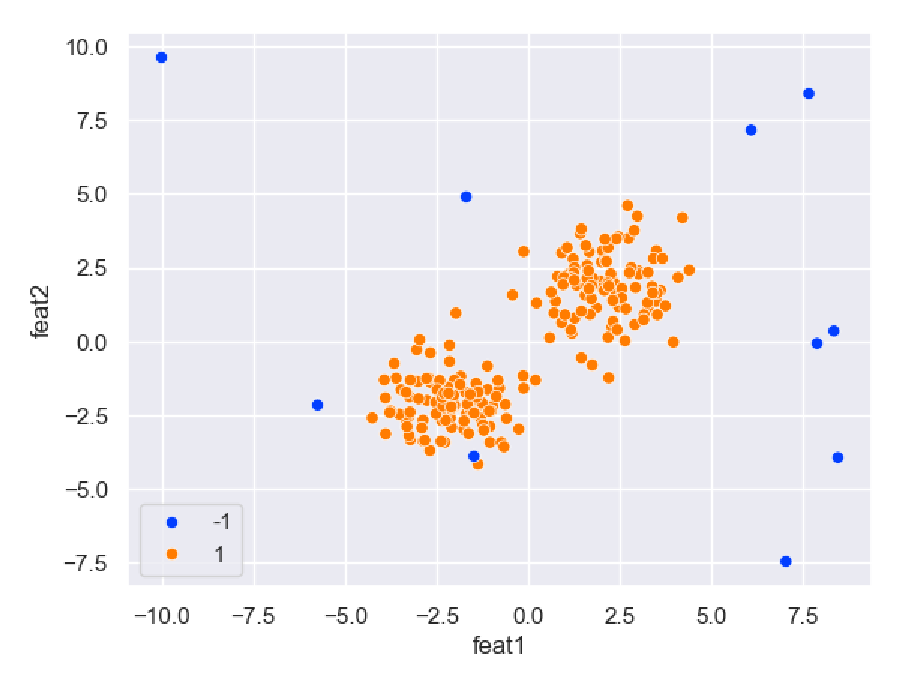
\includegraphics[width=\linewidth]{pictures/eps/demodata.eps}
    \caption{デモデータに関する図の説明(和文)}
    \ecaption{Description of the dim\_vs\_accu figure (English).}
    \label{fig:demodata}
\end{figure}

\subsubsection{特徴量数と精度の関係}
はじめに、デモデータと特徴量数の関係を調査した.図\ref{fig:dim_vs_accu}に示すように、特徴量数が増えるにつれて、異常検知の精度が単調に向上することがわかった.また、精度ののびは増加に反比例して緩やかになっていることもわかる。ゆえに、IFは目標とする精度に対して十分な特徴量数が存在すると言える。

\begin{figure}[tb]
    \centering
    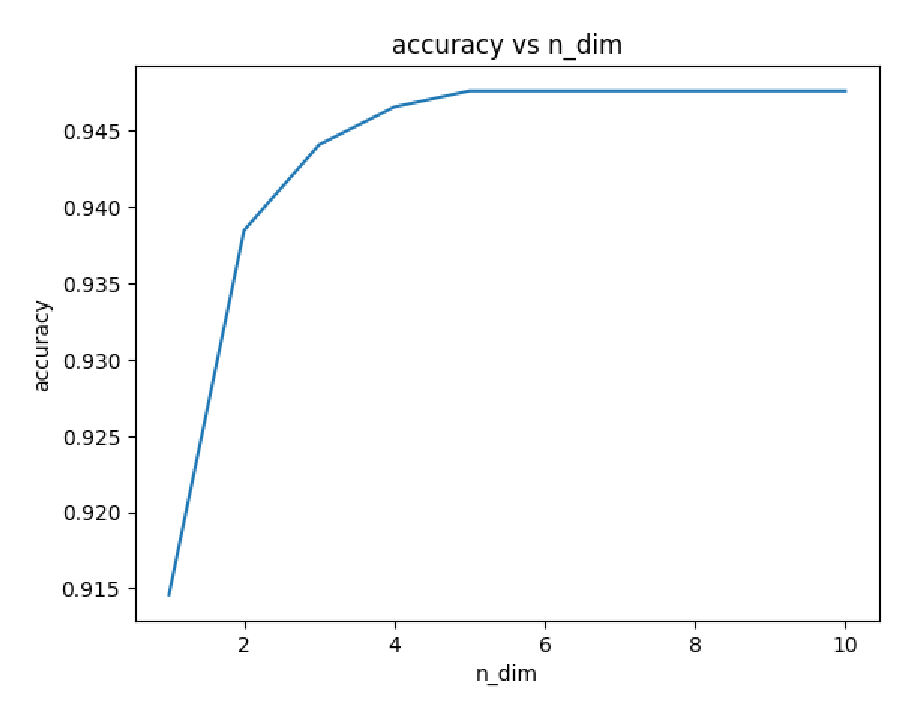
\includegraphics[width=\linewidth]{pictures/eps/dim_vs_accu.eps}
    \caption{dim\_vs\_accuに関する図の説明(和文)}
    \ecaption{Description of the dim\_vs\_accu figure (English).}
    \label{fig:dim_vs_accu}
\end{figure}

\subsubsection{ノイズ特徴量の影響}
続いて、デモデータにノイズ特徴量を含めたときの精度の悪化について調査した。パケット通信を監視して得られたデータセットの全ての特徴が、異常検知に有効なわけではない。そして、IFは特徴量同士の重みづけを行わないため、判定に有効でない特徴量が混ざると精度が低下すると考えられる。図\ref{fig:noise_accu}に示すように、ノイズとなる特徴量が混ざると精度が低下することがわかった。また、今回の実験の場合だと、ノイズ特徴量が判定に有効な特徴量数の2倍以上になると、精度が急激に低下することがわかった。

\begin{figure}[tb]
    \centering
    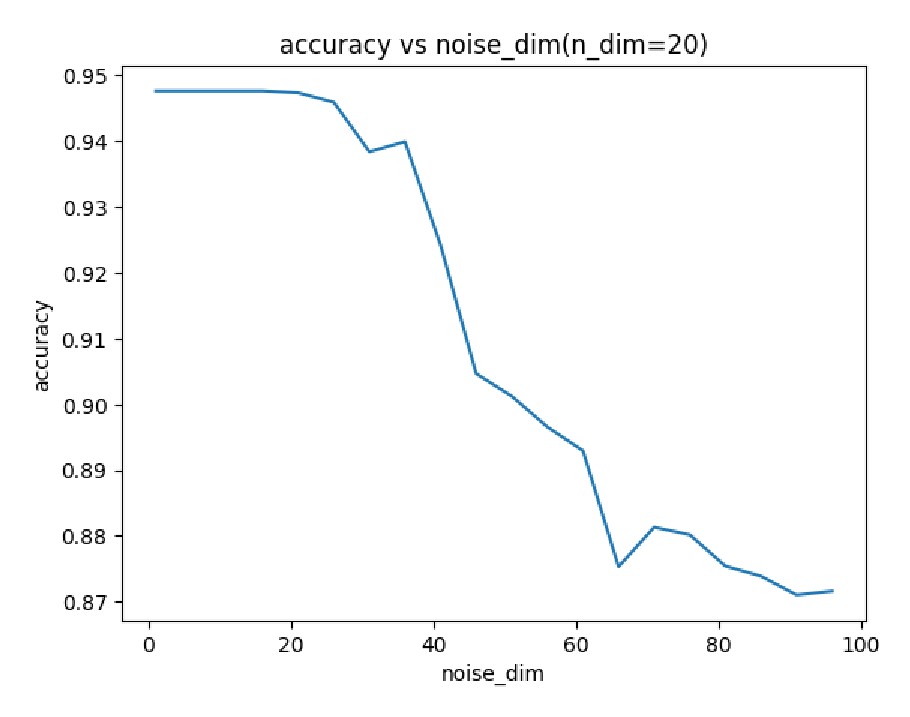
\includegraphics[width=\linewidth]{pictures/eps/noise_accu.eps}
    \caption{noise\_accuに関する図の説明(和文)}
    \ecaption{Description of the noise\_accu figure (English).}
    \label{fig:noise_accu}
\end{figure}

\subsubsection{重要度に基づいたノイズ特徴量の除去}
前の実験から、データセットからノイズとなる特徴量を取り除くことが重要であると考えられる。ところで、IFはツリーベースの異常検知手法である。そこで、同じくツリーベースのRandam Forestから特徴の重要度を算出すれば、ノイズとなる特徴量を取り除けるのではないかと考えた。図\ref{fig:select_noise}は、Random Forestで算出した特徴量の重要度を表している。このグラフは、ノイズ特徴量を判別できていることがわかる。そして、実際にノイズ特徴量を取り除いた場合の精度を調査したところ、精度は???\%から0.945\%まで向上した。この結果から、Feature Importanceによる特徴量選択手法は精度の向上に有効ではないかと考えた。

\begin{figure}[tb]
    \centering
    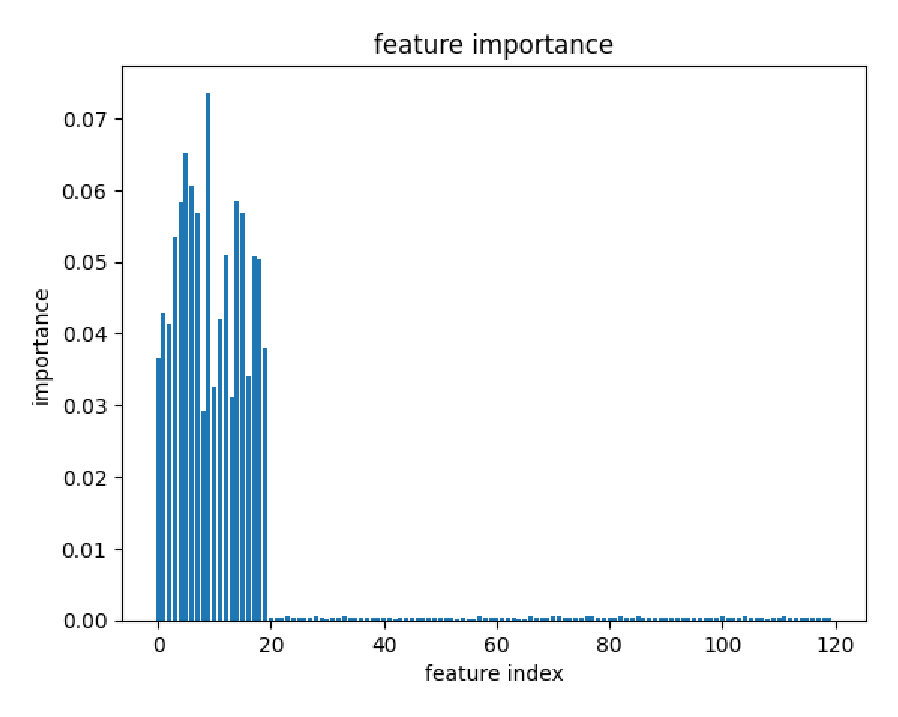
\includegraphics[width=\linewidth]{pictures/eps/select_noise.eps}
    \caption{select\_noiseに関する図の説明(和文)}
    \ecaption{Description of the select\_noise figure (English).}
    \label{fig:select_noise}
\end{figure}

\subsection{異常検知の境界線の問題}
IFを用いた異常検知手法では、攻撃データと正常データのそれぞれでトレーニングされたサブシステムが異常スコアを算出し、これらの結果を組み合わせて最終的な判定を行う。AbuAlgahamらの研究では、表\ref{tab:combination}のようにそれぞれの判定器の結果を組み合わせて判定を行っていた。

\begin{table}[tb]
    \caption{組み合わせアルゴリズム(和文)}
    \ecaption{combination algorithm (English).}
    \centering
    \footnotesize
    \begin{tabular}{ccc}
        \hline
        正常サブシステム & 攻撃サブシステム & 判定結果\\
        \hline
        Normal & Anomaly & Normal \\
        Anomaly & Normal & Anomaly \\
        Normal & Normal & Anomaly \\
        Anomaly & Anomaly & unknown \\
        \hline
    \end{tabular}
    \label{tab:combination}
\end{table}

しかし、表\ref{tab:combination}のようなマッピングに基づく判定手法は、以下の2つの問題を抱えている。
\begin{itemize}
\item 各判定器の異常スコアの閾値を手動で設定する必要があること。
\item 異常判定の境界線が垂直であるため、異常スコアの分布によっては誤判定が多くなること。
\end{itemize}
実際に異常スコアの分布を調査したところ、図\ref{fig:UNSW1}と図\ref{fig:NSL1}で示されるように、異常データと正常データの境界線は対角方向であることが確認された。このような場合、垂直に分割しては正確な判定ができない。

そこで、本研究では、異常スコアの分布に応じて適切な判定ができるよう、異常検知の境界線をロジスティック回帰を用いて決定する手法を提案する。この手法では、それぞれのサブシステムの異常スコアを入力とし、ロジスティック回帰によって最終的な判定を行う。この手法を用いることで、IFの閾値を設定する必要がなく、閾値による垂直な分割よりも正確な判定が行えるという利点がある。

\section{結果と考察}

\subsection{比較するアルゴリズム}

本研究では、以下の2つの比較を行った。
特徴量エンジニアリングの効果の比較を行うため、特徴量選択を行わなかった場合と、Random Forestを用いた特徴量選択手法を用いた場合の結果を比較する。また、判定の組み合わせアルゴリズムの比較には、2つのサブシステムの結果をマッピングする手法と、Rogistic Regressionを用いて判定を行う手法の結果を比較した。

\begin{enumerate}
    \item \textbf{特徴量エンジニアリングの比較}
        \begin{itemize}
            \item 特徴量選択なし
            \item Random Forestを用いた特徴量選択手法
        \end{itemize}
    \item \textbf{判定の組み合わせアルゴリズムの比較}
        \begin{itemize}
            \item 2つのサブシステムの判定を組み合わせて判定
            \item ロジスティック回帰を用いて判定
        \end{itemize}
\end{enumerate}

\subsubsection{実験環境}

実験はMac Book Pro 2017 2.3GHz Intel Core i5, 8GB RAMで行った。また、実験に用いたプログラムはPython3.10.4で実装した。Isolation ForestやRandom Forestの実装には、scikit-learnのライブラリ\footnote[1]{https://scikit-learn.org/stable/}を用いた。

\subsubsection{データセット}
本実験では、以下の2つのデータセットを用いた。

\begin{enumerate}
    \item \textbf{NSL-KDD}
        KDDCUP99の問題点を解決するために提案されたデータセットであり、データの冗長性や攻撃データの割合を調整したもの。
    \item \textbf{UNSW-NB15}
        既存のデータセットの問題点を解決し、現代のネットワークトラフィックと低フットプリント攻撃を包括的に反映するために作成されたデータセット。
\end{enumerate}

\subsubsection{評価指標}
本研究では、以下の2つの評価指標を用いてモデルの性能を評価した。

\begin{enumerate}
    \item \textbf{Accuracy}
        正確度を示し、予測が実際のクラスと一致する割合を示す。
    \item \textbf{F1-score}
        PrecisionとRecallの調和平均を示す。
\end{enumerate}

\subsection{結果}

\subsubsection{異常スコアの分布}
はじめに、2つのデータセットに対してトレーニングデータの異常スコアの分布を調査した。図\ref{fig:UNSW1}はデータセットUNSWにおける異常スコアの分布を示し、図\ref{fig:NSL1}はデータセットNSLにおける異常スコアの分布を示し。横軸は正常データで訓練されたIFが算出した異常スコアを表し、縦軸は攻撃データで訓練されたIFが計算した異常スコアを表している。それぞれのゼロ点は異常スコアの閾値であり、負の方向に大きくなるほど異常スコアが高く、正の方向に大きくなるほど異常スコアが低いことを意味する。各データ点の色はラベルを示しており、赤が攻撃データ(1)、青が正常データ(0)を表す。

図\ref{fig:UNSW1}をみると、UNSWデータセットではデータが対角線方向に分布しており、2つのサブシステムの判定が相反する場合が多いことがわかる。また、右下に正常データが多く存在し、この領域の判定は適切に行われていることもわかる。攻撃データと正常データの境界線が対角方向に位置しているため、従来の垂直な分割に比べて、ロジスティック回帰を用いて斜めに分割することで精度が向上する可能性がある。

図\ref{fig:NSL1}から、データセットNSLでは、右下と左下にそれぞれ攻撃データと正常データが集中しており、適切に行われている判定が多いことがわかる。同様に、2つのデータの境界線が対角線方向に位置しているため、ロジスティック回帰を用いることで精度が向上する可能性がある。

\begin{figure}[tb]
    \centering
    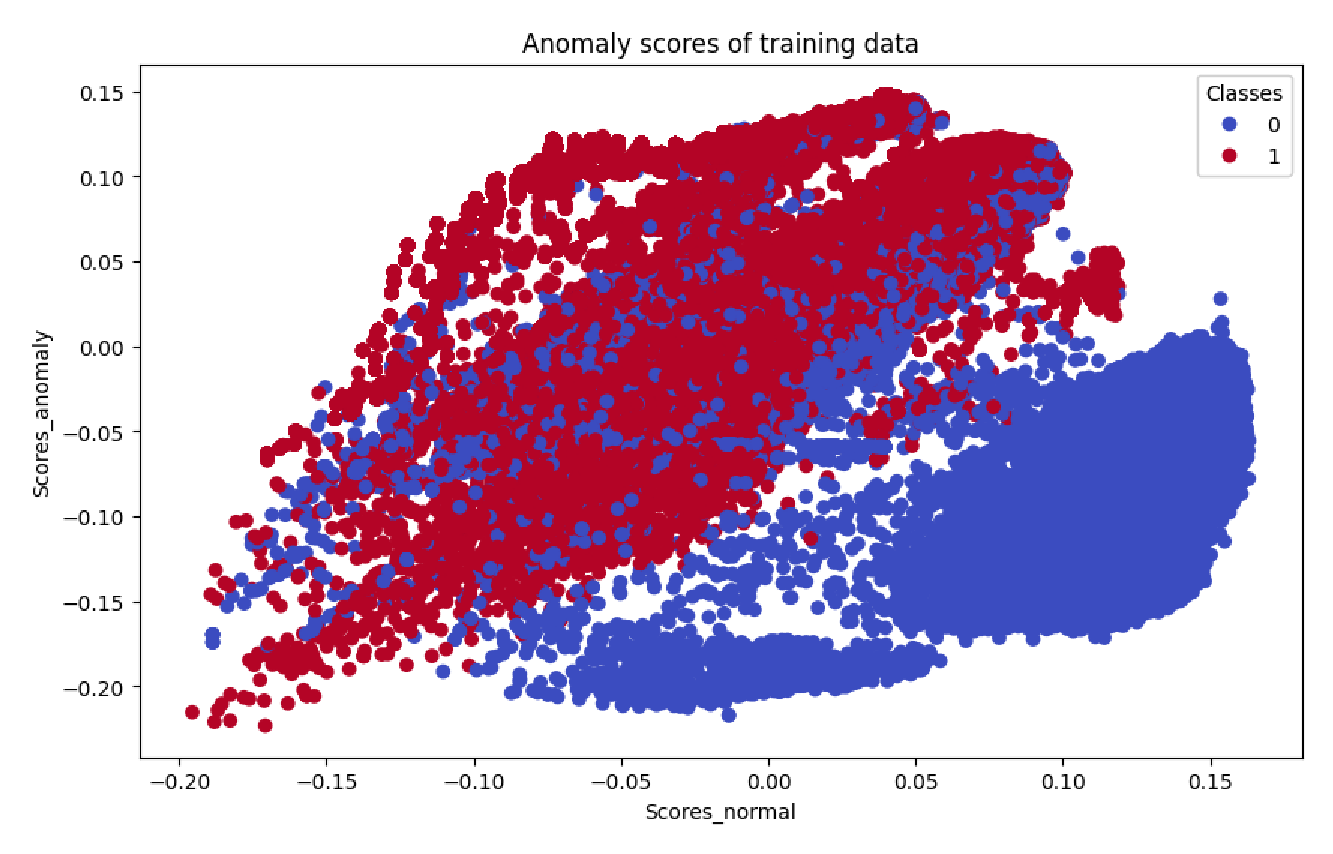
\includegraphics[width=\linewidth]{pictures/eps/UNSW1.eps}
    \caption{UNSW1(和文)}
    \ecaption{Description of the collectness\_UNSW figure (English).}
    \label{fig:UNSW1}
\end{figure}

\begin{figure}[tb]
    \centering
    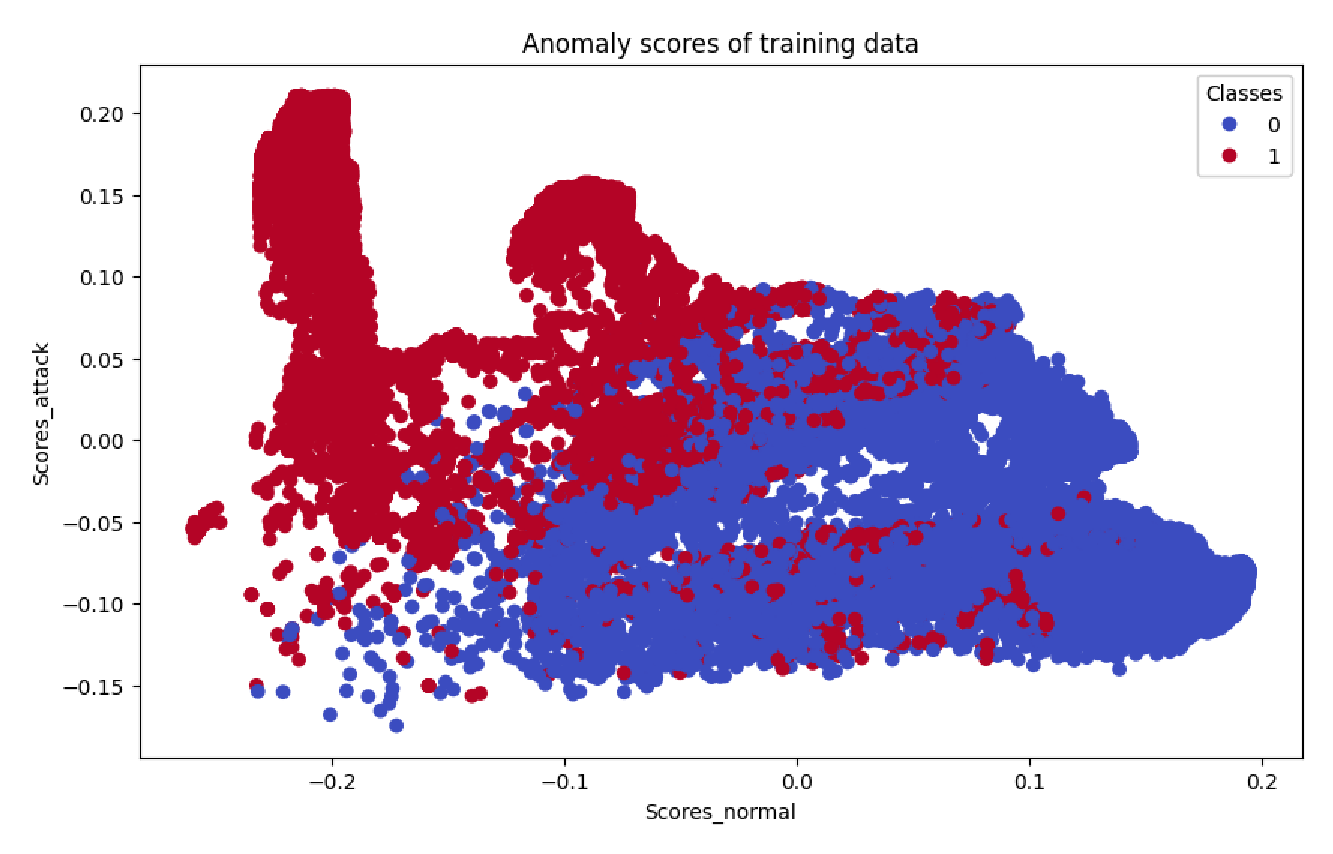
\includegraphics[width=\linewidth]{pictures/eps/NSL1.eps}
    \caption{NSL1(和文)}
    \ecaption{Description of the collectness\_UNSW figure (English).}
    \label{fig:NSL1}
\end{figure}

\begin{table}[tb]
    \caption{UNSWでのモデルの性能評価結果(和文)}
    \ecaption{Performance evaluation results of models in UNSW Dataset(English).}
    \centering
    \footnotesize
    \begin{tabular}{lcccc}
        \hline\hline
        Model & Accuracy & F1 \\
        \hline
        特徴量選択なし & 0.7506 & 0.7526 \\
        特徴量選択なし, 提案手法 & 0.8685 & 0.8666 \\
        特徴量選択あり & 0.8440 & 0.8817 \\
        特徴量選択あり, 提案手法 & 0.9112 & 0.9082 \\
        \hline
    \end{tabular}
    \label{tab:model_performance_UNSW}
\end{table}

\begin{table}[tb]
    \caption{NSLでのモデルの性能評価結果(和文)}
    \ecaption{Performance evaluation results of models in NSL Dataset(English).}
    \centering
    \footnotesize
    \begin{tabular}{lcc}
        \hline\hline
        Model & Accuracy & F1 \\
        \hline
        特徴量選択なし & 0.7873 & 0.8171 \\
        特徴量選択なし、提案手法 & - & -\\ 
        特徴量選択あり & 0.8466 & 0.8775 \\
        特徴量選択あり、提案手法 & 0.9452 & 0.9452 \\
        \hline
    \end{tabular}
    \label{tab:model_performance_NSL}
\end{table}

\subsubsection{モデルの性能評価}
それぞれの実験結果は表\ref{tab:model_performance_UNSW},表\ref{tab:model_performance_NSL}の通りである。表\ref{tab:model_performance_UNSW}を見ると、特徴量の選択をすることで、精度が0.7506から0.8440に向上したことがわかる。また、ロジスティック回帰を用いて判定を行うことで、精度が0.8440から0.9112に向上したことがわかる。同様に、表\ref{tab:model_performance_NSL}から、データセットNSLでも、特徴量の選択をすることで精度が0.7873から0.8466に向上し、ロジスティック回帰を用いて判定を行うことで精度が0.8466から0.9452に向上したことが確認できた。

\subsection{考察}

\begin{figure}
    \centering
    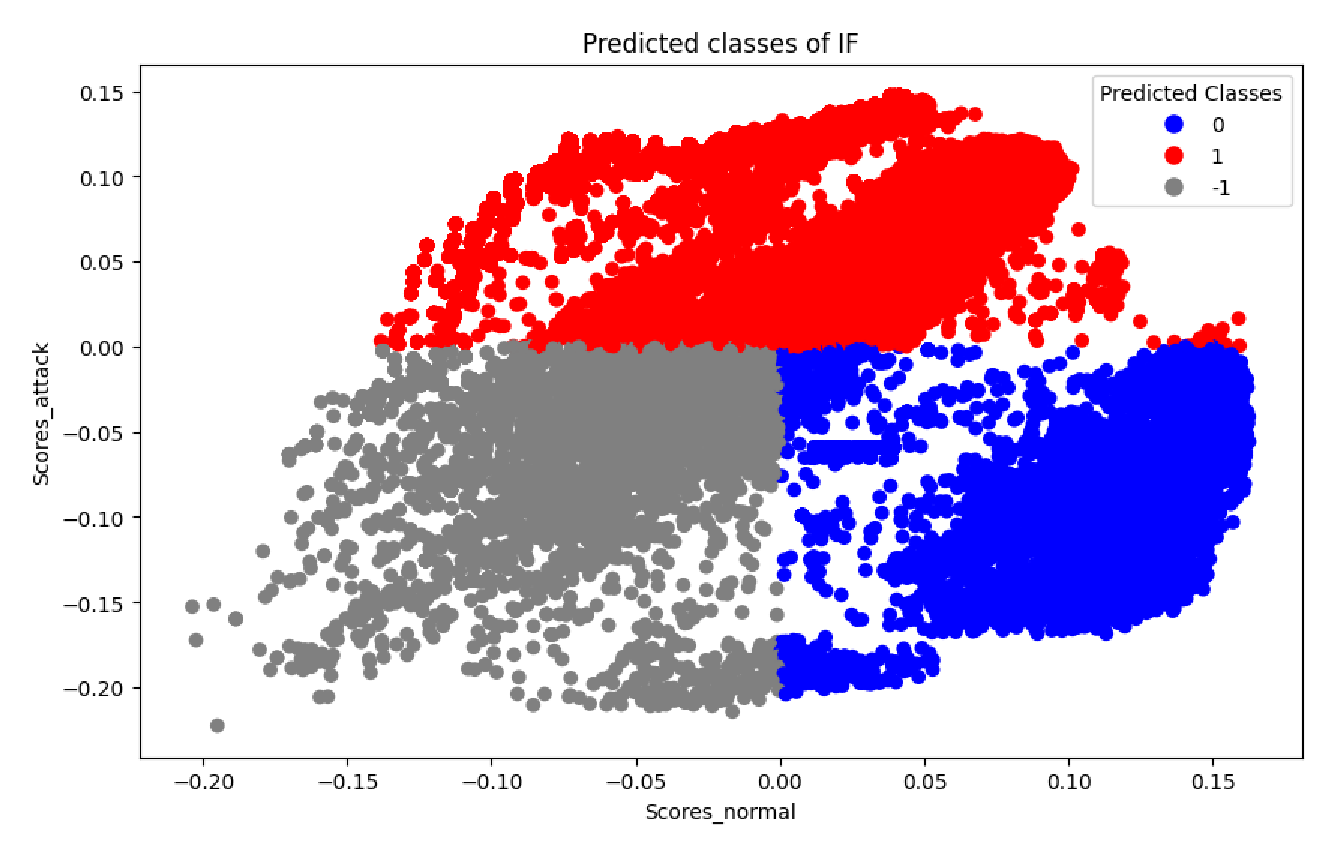
\includegraphics[width=\linewidth]{pictures/eps/UNSW2.eps}
    \caption{UNSW2(和文)}
    \ecaption{Description of the collectness\_UNSW figure (English).}
    \label{fig:UNSW2}
\end{figure}

\begin{figure}
    \centering
    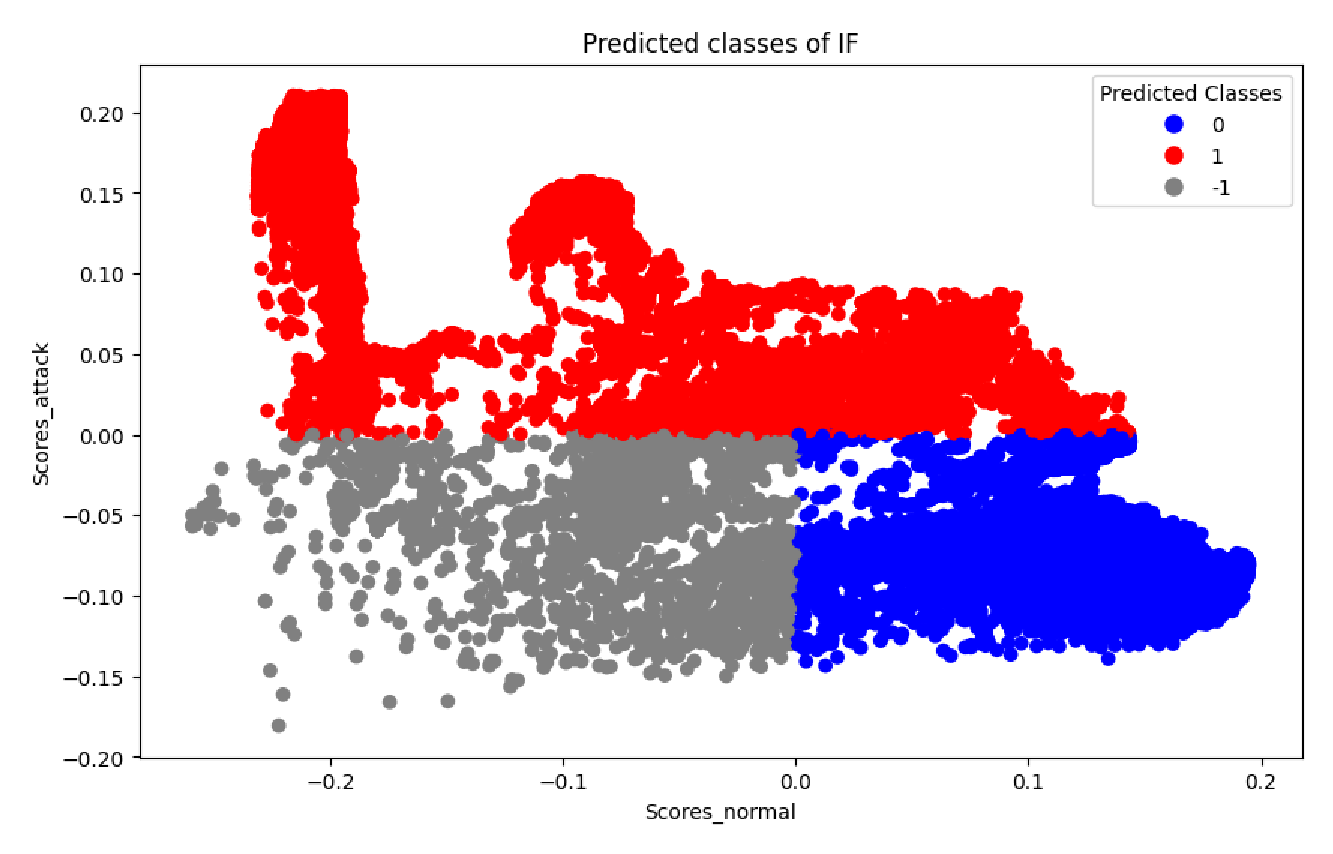
\includegraphics[width=\linewidth]{pictures/eps/NSL2.eps}
    \caption{NSL2(和文)}
    \ecaption{Description of the collectness\_UNSW figure (English).}
    \label{fig:NSL2}
\end{figure}

\begin{figure}
    \centering
    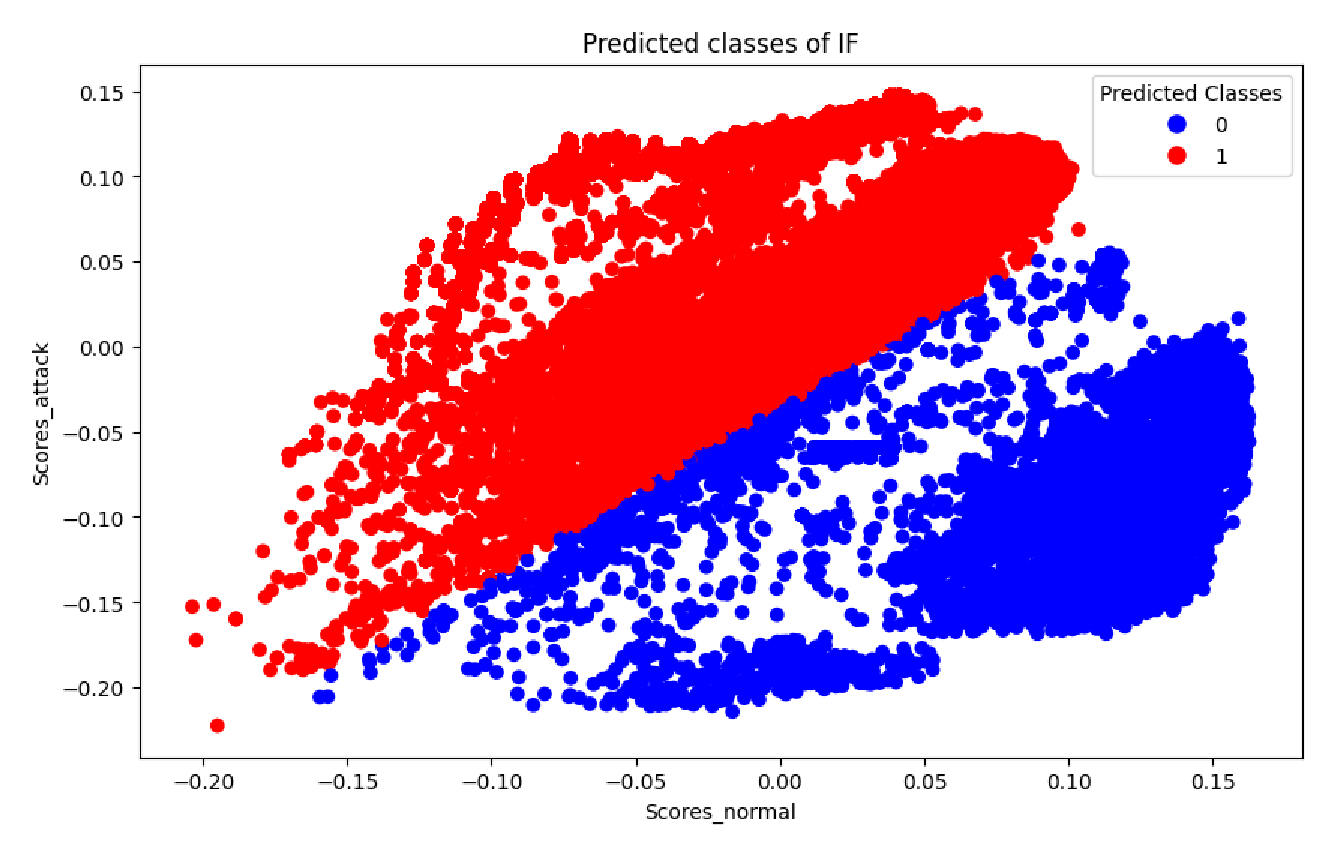
\includegraphics[width=\linewidth]{pictures/eps/UNSW3.eps}
    \caption{UNSW3(和文)}
    \ecaption{Description of the collectness\_UNSW figure (English).}
    \label{fig:UNSW3}
\end{figure}

\begin{figure}
    \centering
    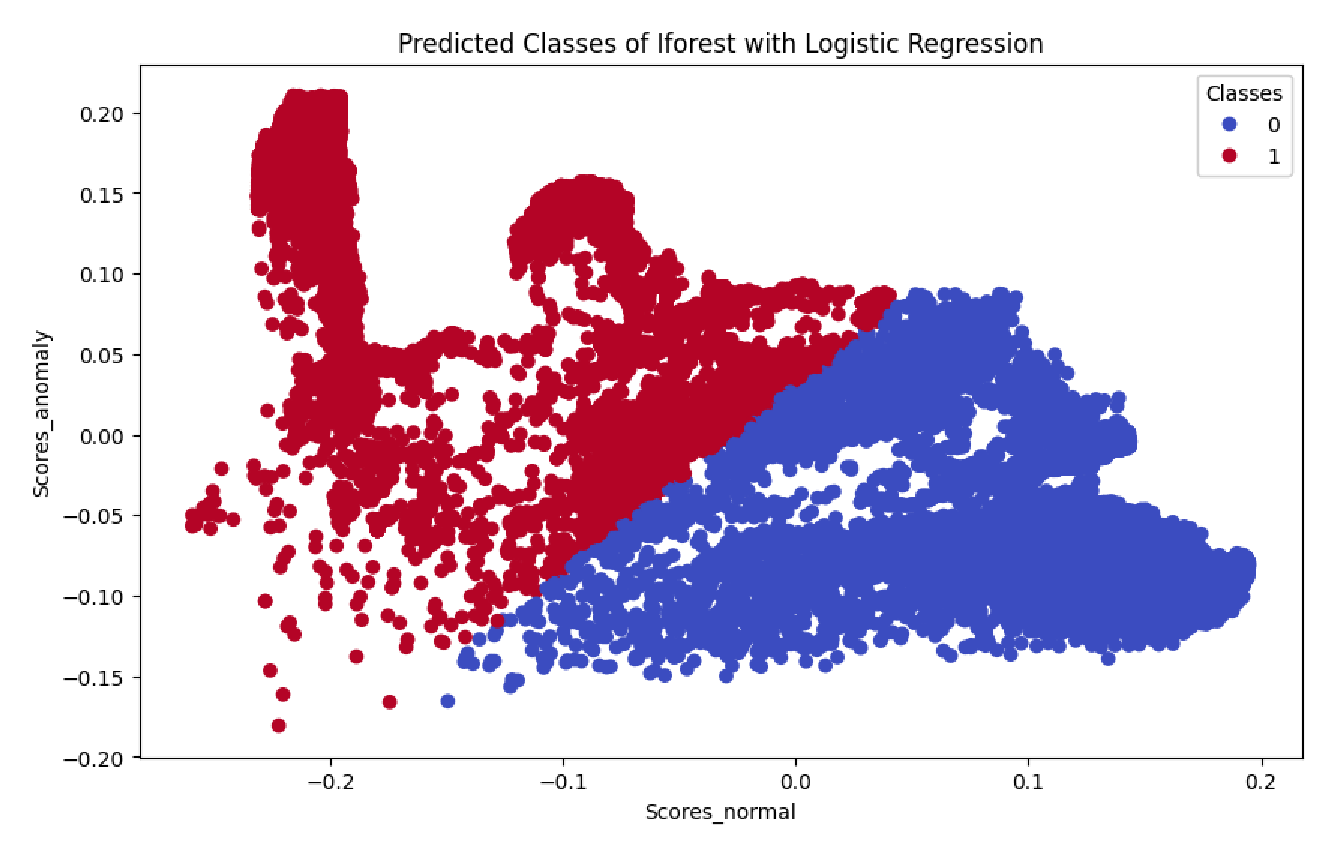
\includegraphics[width=\linewidth]{pictures/eps/NSL3.eps}
    \caption{NSL3(和文)}
    \ecaption{Description of the collectness\_UNSW figure (English).}
    \label{fig:NSL3}
\end{figure}

まず、ロジスティック回帰を導入することで、異常スコアの分布が斜めに広がる場合にもより正確な境界を引くことが可能になった。図\ref{fig:UNSW2}と図\ref{fig:NSL2}はそれぞれ、2つのサブシステムの判定結果を組み合わせた手法の結果を示しており、図\ref{fig:UNSW3}と図\ref{fig:NSL3}はロジスティック回帰を用いた手法の結果を示している。図\ref{fig:UNSW2}と図\ref{fig:NSL2}からは、2つのサブシステムの判定を組み合わせた手法では、どれだけ閾値を適切に設定したとしても、異常スコアの分布が斜めに広がる場合には誤判定が多く発生することがわかる。一方、図\ref{fig:UNSW3}と図\ref{fig:NSL3}からは、ロジスティック回帰を用いた手法が斜めに広がる異常スコアの分布に対してもより正確な判定が可能であることが確認される。これにより、従来の垂直な分割では誤判定が多発するケースにおいても、精度の向上が見込めることが実証された。

また、今回のアプローチが適用できる範囲についても考察が必要である。異常スコアの分布が明確に分かれている場合にはこの手法が効果的であるが、攻撃通信と正常通信が十分に分離されていない場合や、異常スコアの境界線が曲面状になっている場合には、別の特徴量選択手法の採用や異なる機械学習アルゴリズムの適用など、さらなる工夫が必要とされる。実際、図\ref{fig:UNSW1}と図\ref{fig:NSL1}で示される2つのデータセットを比較すると、NSLデータセットはUNSWデータセットよりも攻撃通信と正常通信が明確に分離されていることが観察される。その結果、検知精度に関しても、NSLデータセットはUNSWデータセットに対して高い精度を示している。このことから、異常スコアの分布が明確に分かれている場合には、提案手法が有効であることが示唆される。

さらに、ロジスティック回帰を適用する際のコストや計算量に関するトレードオフも存在する。IF単体での異常検知に比べ、ロジスティック回帰を用いることでモデル構築にかかる計算時間が増加することが懸念される。


また、異なるデータセットや環境における適用性についても、今後の研究課題として残されている。

以上より、提案手法は特定の条件下では高い効果を発揮することが確認されたが、全てのシナリオにおいて万能であるとは限らない。今後は、異常スコアの分布がさらに複雑な場合における改良や、計算効率の最適化について検討することが求められる。

\section{おわりに}
おわりにを書く.

\begin{acknowledgment}
謝辞を書く.\cite{AbuAlghanam2023-sx}
\end{acknowledgment}


\bibliographystyle{junsrt} % 参照順
\bibliography{references}

\end{document}
